\chapter{Estruturas de Dados para Inteiros}

Neste capítulo, voltamos ao problema de implementar um #SSet#.
A diferença agora é que assumimos que os elementos armazenados no #SSet# são inteiros com #w#-bits. Ou seja, queremos implementar #add(x)#, #remove(x)#, e #find(x)# onde $#x#\in\{0,\ldots,2^{#w#}-1\}$. Não é muito difícil	pensar em muitas aplicações em que os dados---ou pelo menos a chave que usamos para classificar os dados---é um número inteiro.

Discutiremos três estruturas de dados, cada uma com base nas idéias da anterior. A primeira estrutura, a #BinaryTrie# executa todas as três operações de um #SSet# em um tempo $O(#w#)$. Isso não é muito impressionante, pois qualquer subconjunto de $\{0,\ldots,2^{#w#}-1\}$ tem o tamanho $#n#\le 2^{#w#}$, para que $\log #n# \le #w#$. Todas as outras implementações de #SSet# discutidas neste livro realizam todas as operações em um tempo $O(\log #n#)$, para que sejam todas pelo menos tão rápidas quanto uma #BinaryTrie#.

The second structure, the #XFastTrie#, speeds up the search in a
#BinaryTrie# by using hashing.  With this speedup, the #find(x)#
operation runs in $O(\log #w#)$ time.  However, #add(x)# and #remove(x)#
operations in an #XFastTrie# still take $O(#w#)$ time and the space used
by an #XFastTrie# is $O(#n#\cdot#w#)$.

The third data structure, the #YFastTrie#, uses an #XFastTrie# to store
only a sample of roughly one out of every $#w#$ elements and stores the
remaining elements in a standard #SSet# structure.  This trick reduces the
running time of #add(x)# and #remove(x)# to $O(\log #w#)$ and decreases
the space to $O(#n#)$.

The implementations used as examples in this chapter can store any type of
data, as long as an integer can be associated with it.  In the code samples,
the variable #ix# is always the integer value associated with #x#, and the method \javaonly{#in.#}#intValue(x)# converts #x# to its associated integer. In
the text, however, we will simply treat #x# as if it is an integer.

\section{#BinaryTrie#: A digital search tree}
\seclabel{binarytrie}

\index{BinaryTrie@#BinaryTrie#}%
A #BinaryTrie# encodes a set of #w# bit integers in a binary tree.
All leaves in the tree have depth #w# and each integer is encoded as a
root-to-leaf path.  The path for the integer #x# turns left at level #i#
if the #i#th most significant bit of #x# is a 0 and turns right if it
is a 1.  \figref{binarytrie-ex} shows an example for the case $#w#=4$,
in which the trie stores the integers 3(0011), 9(1001), 12(1100),
and 13(1101).
\begin{figure}
  \begin{center}
    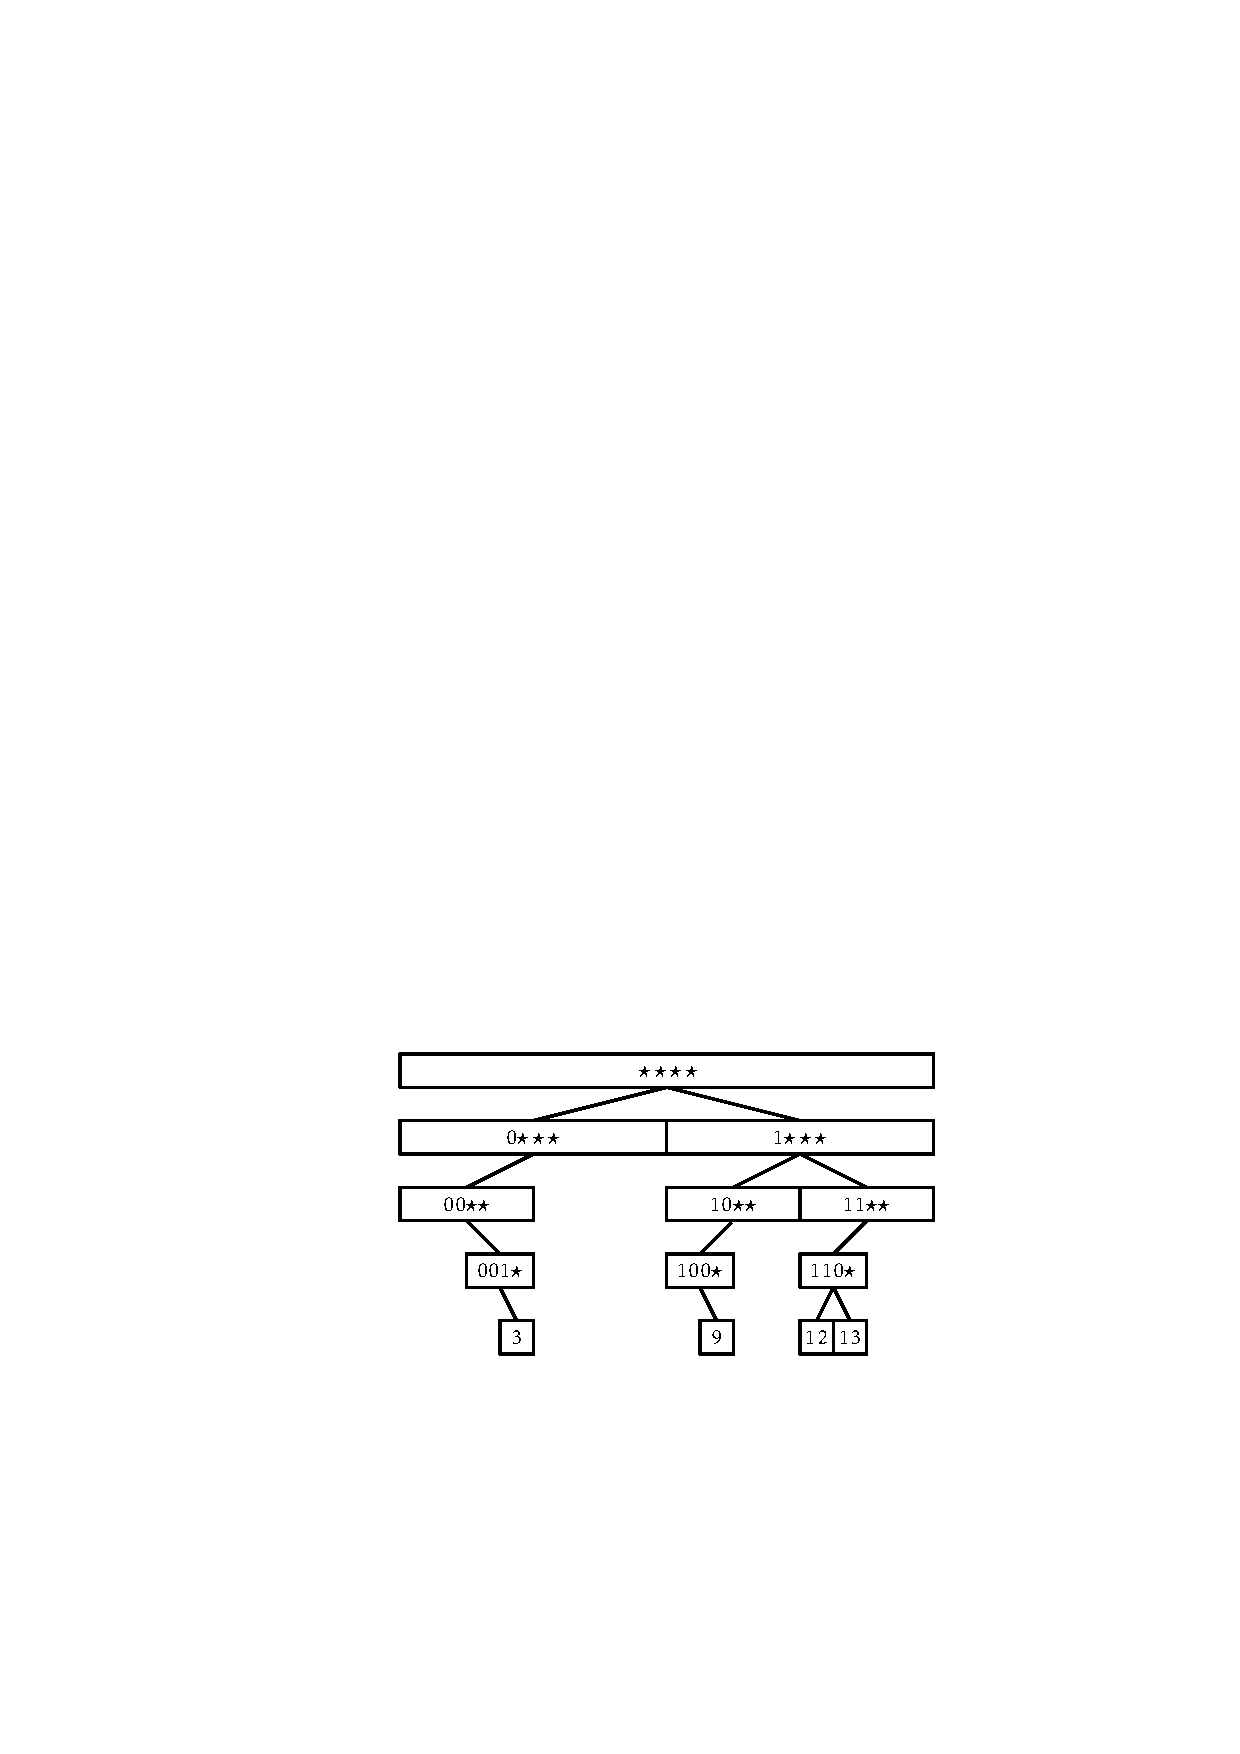
\includegraphics[width=\ScaleIfNeeded]{figs/binarytrie-ex-1}
  \end{center}
  \caption{The integers stored in a binary trie are encoded as
    root-to-leaf paths.}
  \figlabel{binarytrie-ex}
\end{figure}

Because the search path
\index{search path!in a #BinaryTrie#}%
for a value #x# depends on the bits of #x#, it will
be helpful to name the children of a node, #u#, #u.child[0]# (#left#)
and #u.child[1]# (#right#).  These child pointers will actually serve
double-duty.  Since the leaves in a binary trie have no children, the
pointers are used to string the leaves together into a doubly-linked list.
For a leaf in the binary trie #u.child[0]# (#prev#) is the node that
comes before #u# in the list and #u.child[1]# (#next#) is the node that
follows #u# in the list.  A special node, #dummy#, is used both before
the first node and after the last node in the list (see \secref{dllist}).
\cpponly{In the code samples, #u.child[0]#, #u.left#, and #u.prev# refer to the same field in the node #u#, as do #u.child[1]#, #u.right#, and #u.next#.}

Each node, #u#, also contains an additional pointer #u.jump#.  If #u#'s
left child is missing, then #u.jump# points to the smallest leaf in
#u#'s subtree.  If #u#'s right child is missing, then #u.jump# points
to the largest leaf in #u#'s subtree.  An example of a #BinaryTrie#,
showing #jump# pointers and the doubly-linked list at the leaves, is
shown in \figref{binarytrie-ex2}.

\begin{figure}
  \begin{center}
    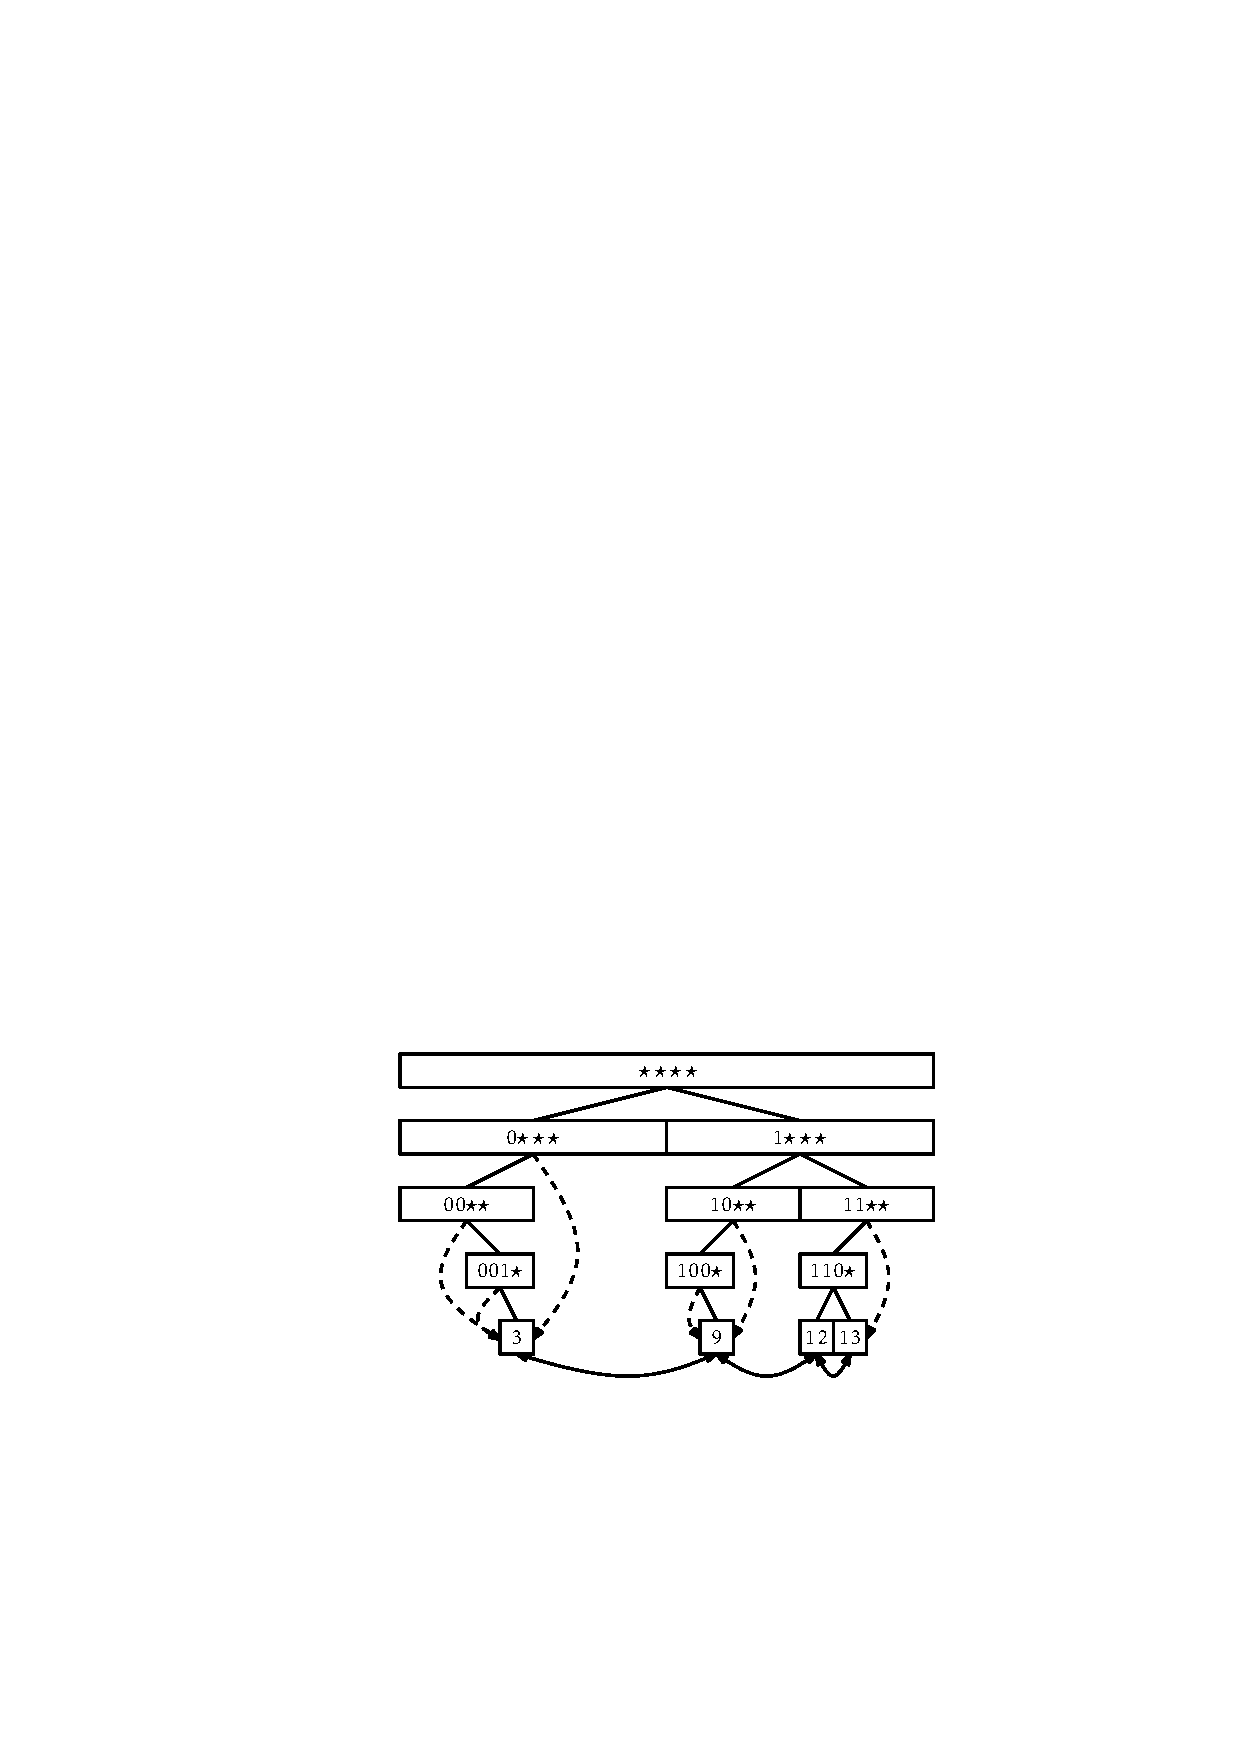
\includegraphics[width=\ScaleIfNeeded]{figs/binarytrie-ex-2}
  \end{center}
  \caption[A BinaryTrie]{A #BinaryTrie# with #jump# pointers shown as curved dashed
  edges.}
  \figlabel{binarytrie-ex2}
\end{figure}


%\jxavaimport{ods/BinaryTrie.Node<Node}
%\cxppimport{ods/BinaryTrie.BinaryTrieNode<Node}

The #find(x)# operation in a #BinaryTrie# is fairly straightforward.
We try to follow the search path for #x# in the trie.  If we reach a leaf,
then we have found #x#.  If we reach a node #u# where we cannot proceed
(because #u# is missing a child), then we follow #u.jump#, which takes us
either to the smallest leaf larger than #x# or the largest leaf smaller than
#x#. Which of these two cases occurs depends on whether #u# is missing
its left or right child, respectively.  In the former case (#u# is missing
its left child), we have found the node we want.  In the latter case (#u#
is missing its right child), we can use the linked list to reach the node
we want. Each of these cases is illustrated in \figref{binarytrie-find}.
\codeimport{ods/BinaryTrie.find(x)}
\begin{figure}
  \begin{center}
    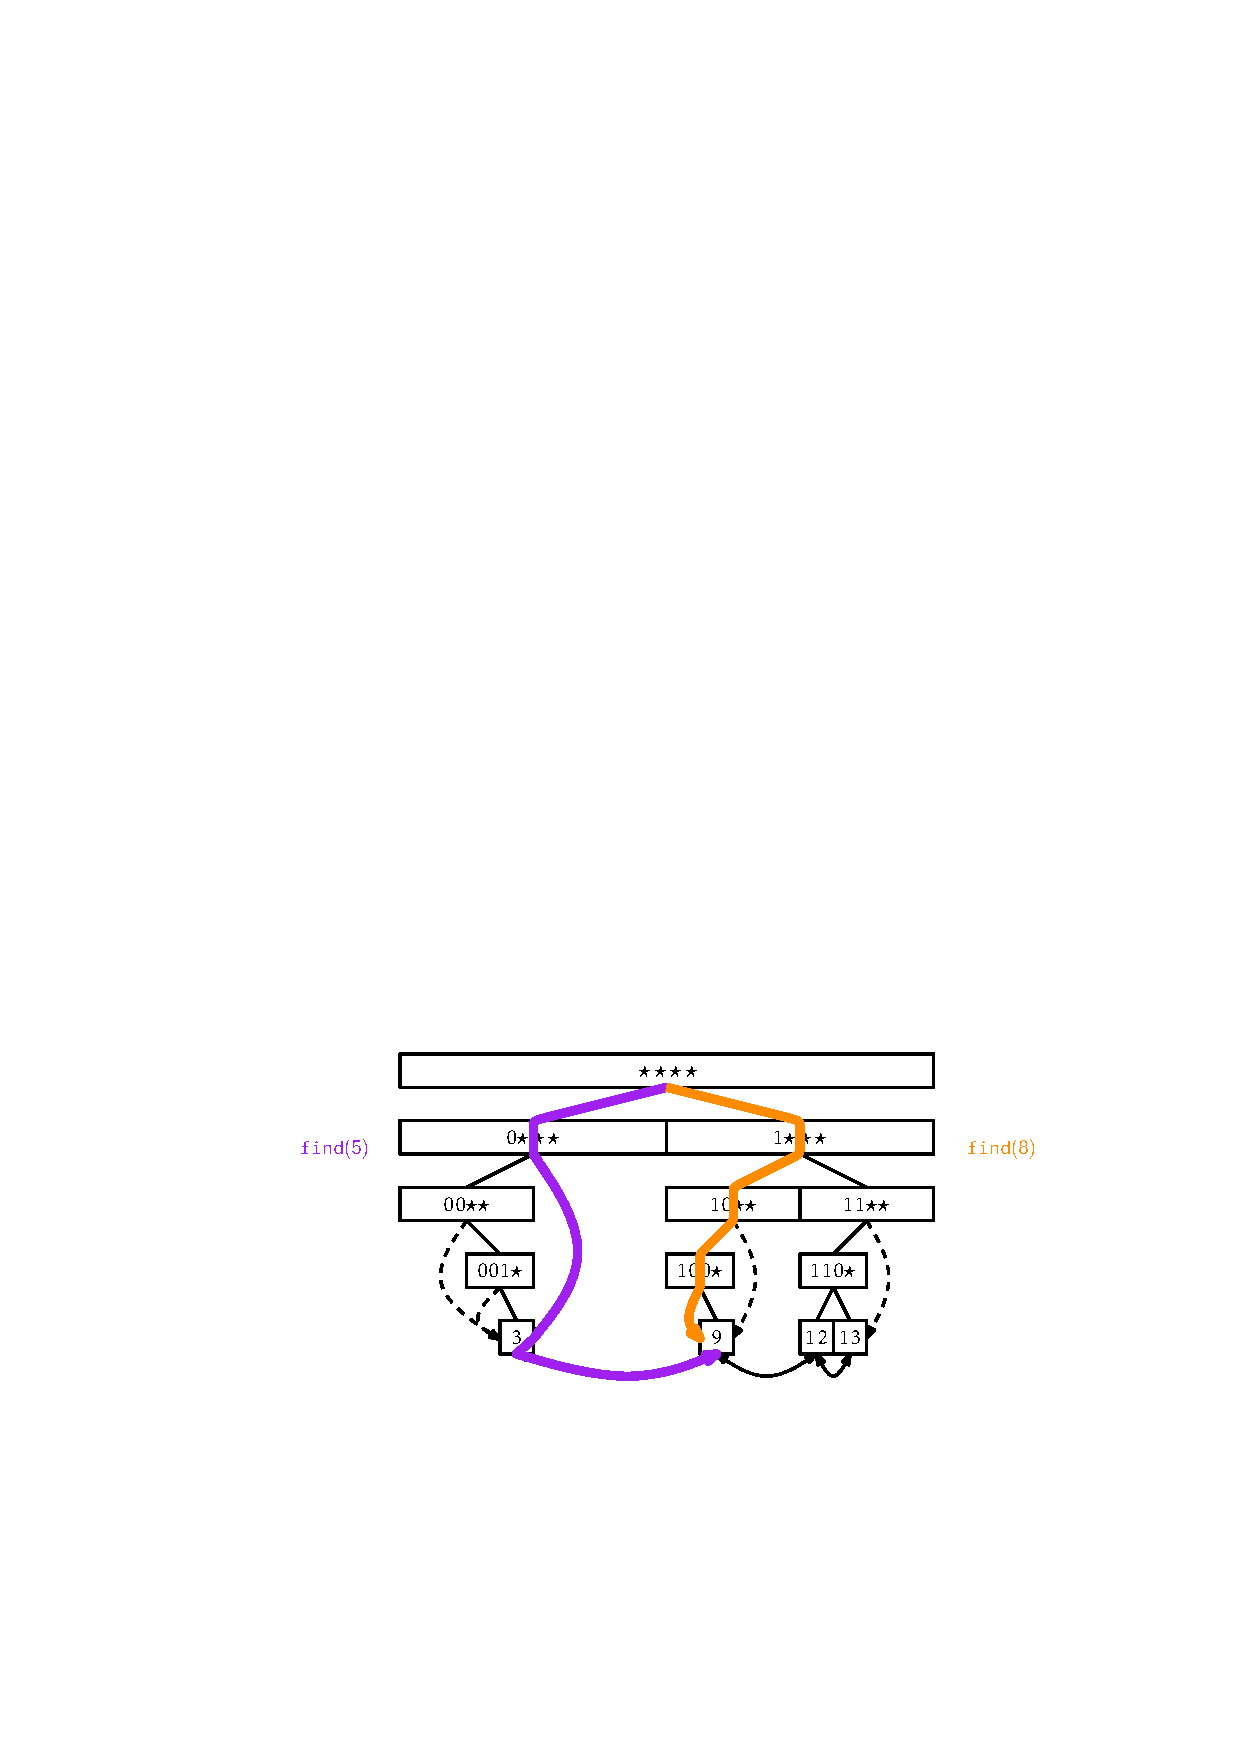
\includegraphics[width=\ScaleIfNeeded]{figs/binarytrie-ex-3}
  \end{center}
  \caption[Search paths in a BinaryTrie]{The paths followed by #find(5)# and #find(8)#.}
  \figlabel{binarytrie-find}
\end{figure}
The running-time of the #find(x)# method is dominated by the time it
takes to follow a root-to-leaf path, so it runs in $O(#w#)$ time.

The #add(x)# operation in a #BinaryTrie# is also fairly straightforward,
but has a lot of work to do:
\begin{enumerate}
  \item It follows the search path for #x# until reaching a node #u#
    where it can no longer proceed.
  \item It creates the remainder of the search path from #u# to a leaf
    that contains #x#.
  \item It adds the node, #u'#, containing #x# to the linked list
    of leaves (it has access to the predecessor, #pred#, of #u'# in
    the linked list from the #jump# pointer of the last node, #u#,
    encountered during step~1.)
  \item It walks back up the search path for #x# adjusting #jump#
    pointers at the nodes whose #jump# pointer should now point to #x#.
\end{enumerate}
An addition is illustrated in \figref{binarytrie-add}.
\begin{figure}
  \begin{center}
    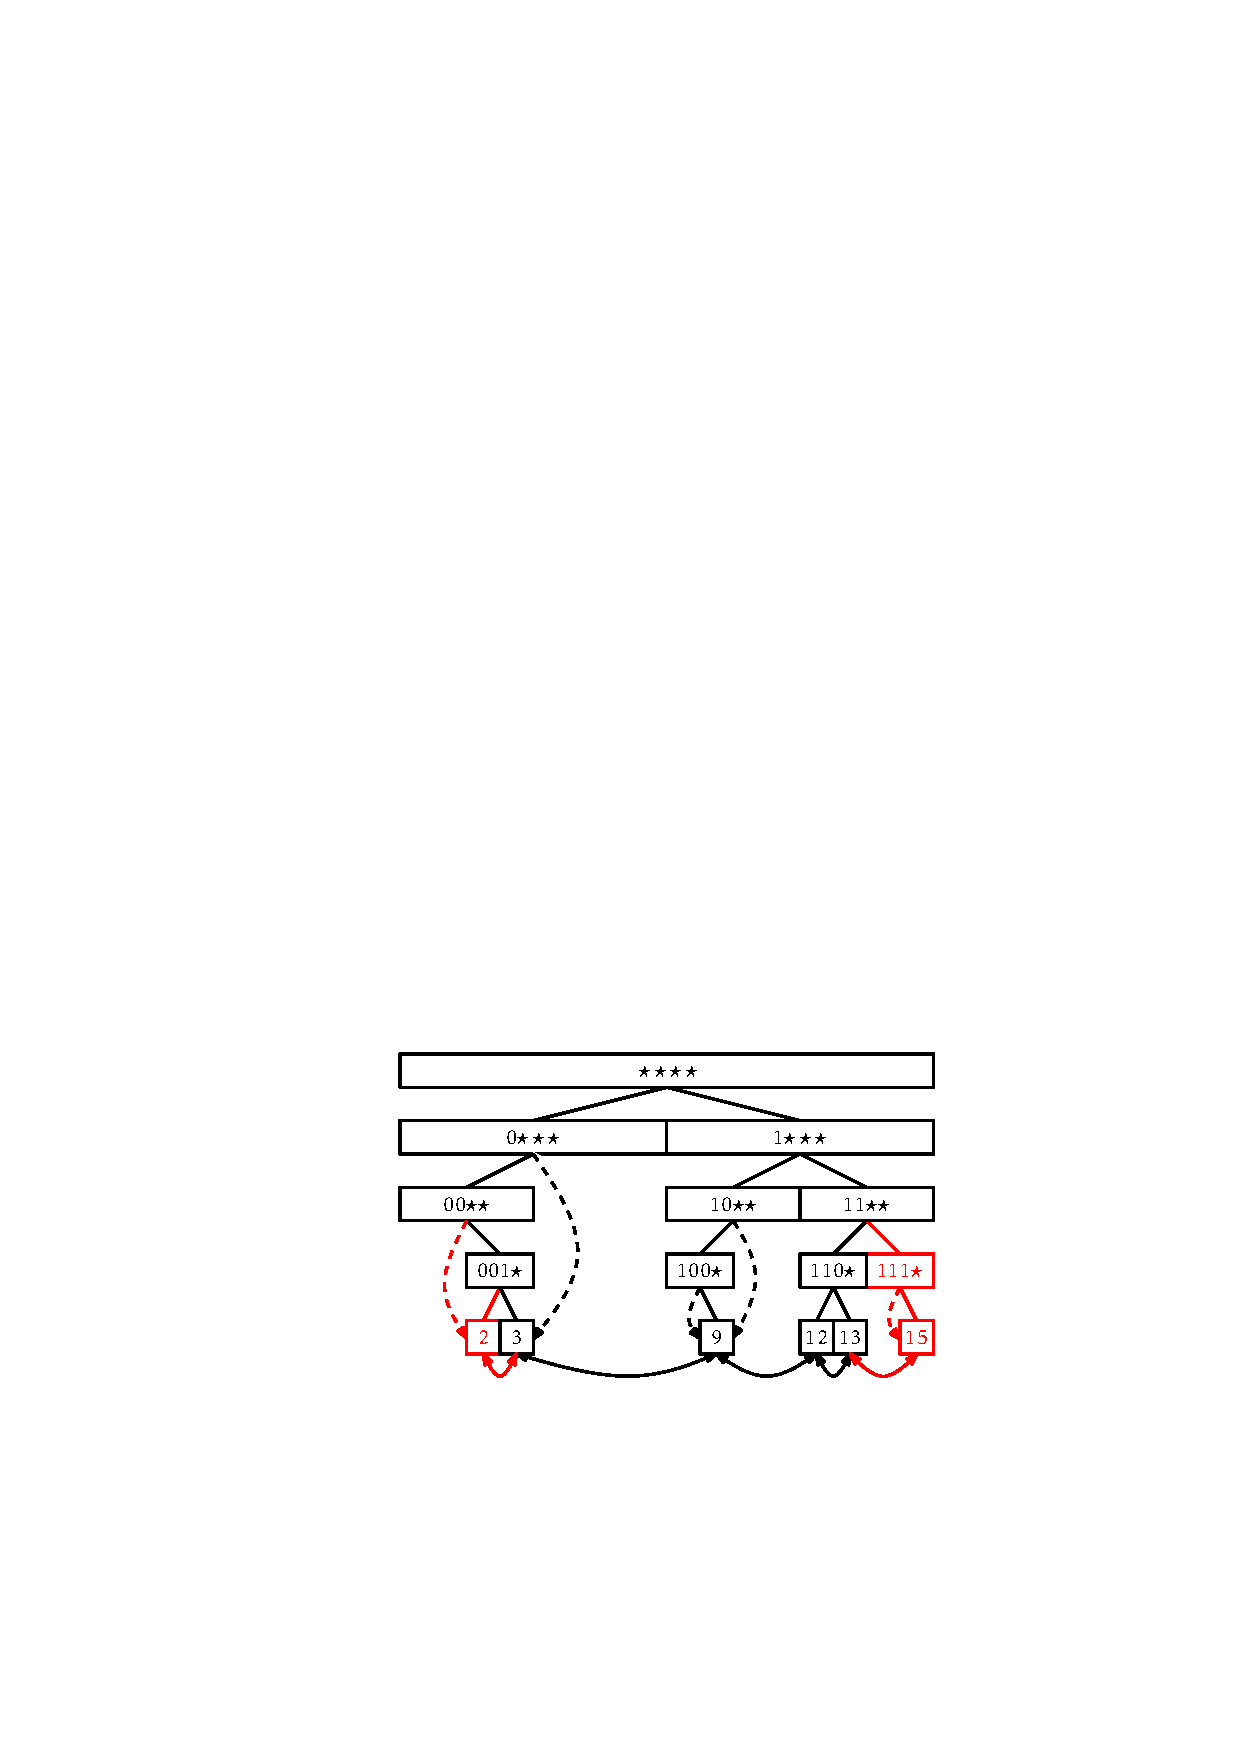
\includegraphics[width=\ScaleIfNeeded]{figs/binarytrie-add}
  \end{center}
  \caption[Adding to a BinaryTrie]{Adding the values 2 and 15 to the #BinaryTrie# in
  \figref{binarytrie-ex2}.}
  \figlabel{binarytrie-add}
\end{figure}
\codeimport{ods/BinaryTrie.add(x)}
This method performs one walk down the search path for #x# and one walk
back up.  Each step of these walks takes constant time, so the #add(x)#
method runs in $O(#w#)$ time.


The #remove(x)# operation undoes the work of #add(x)#.  Like #add(x)#,
it has a lot of work to do:
\begin{enumerate}
  \item It follows the search path for #x# until reaching the leaf, #u#,
  containing #x#.
  \item It removes #u# from the doubly-linked list.
  \item It deletes #u# and then walks back up the search path for #x#
  deleting nodes until reaching a node #v# that has a child that is not
  on the search path for #x#.
  \item It walks upwards from #v# to the root updating any #jump# pointers
  that point to #u#.
\end{enumerate}
A removal is illustrated in \figref{binarytrie-remove}.
\begin{figure}
  \begin{center}
    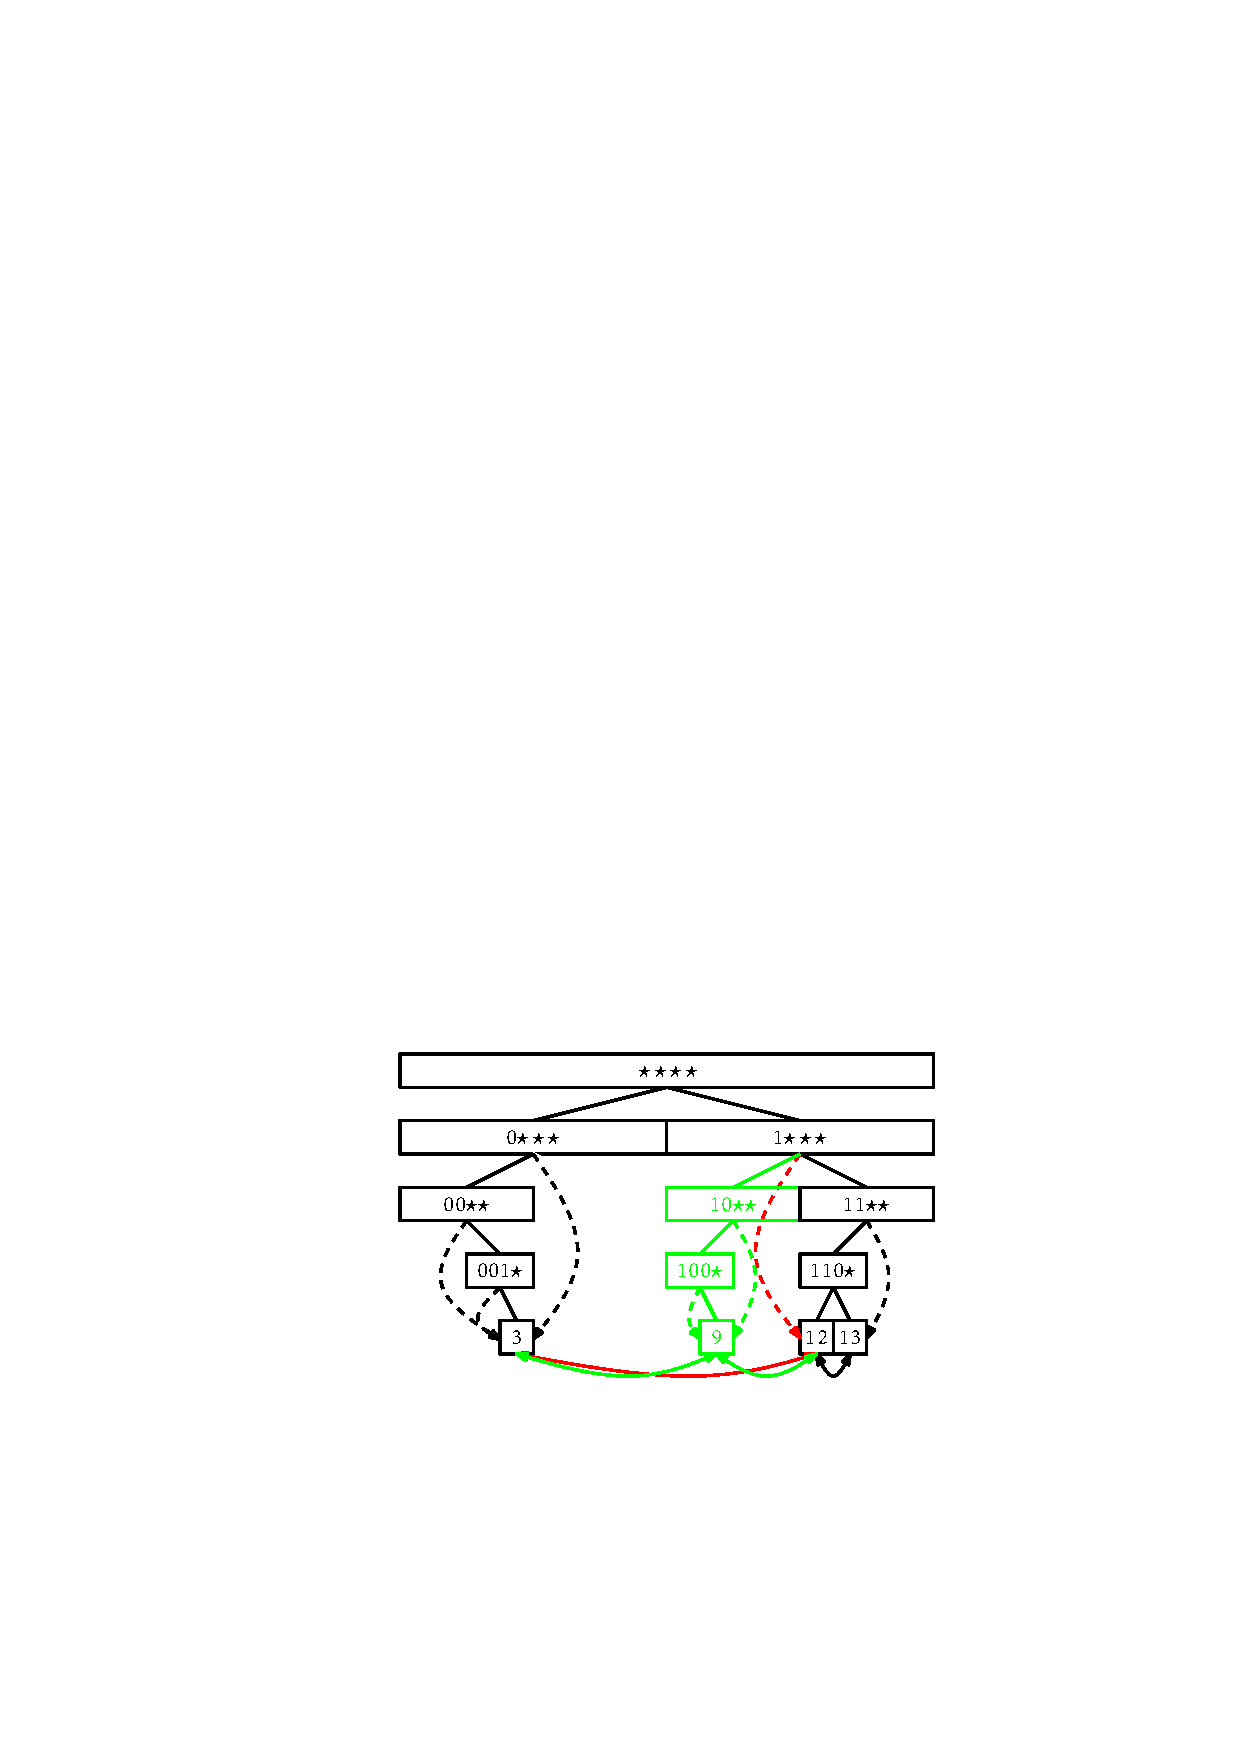
\includegraphics[scale=0.90909]{figs/binarytrie-remove}
  \end{center}
  \caption[Removing from a BinaryTrie]{Removing the value 9 from the #BinaryTrie# in
  \figref{binarytrie-ex2}.}
  \figlabel{binarytrie-remove}
\end{figure}
\codeimport{ods/BinaryTrie.remove(x)}

\begin{thm}
A #BinaryTrie# implements the #SSet# interface for #w#-bit integers. A
#BinaryTrie# supports the operations #add(x)#, #remove(x)#, and #find(x)#
in $O(#w#)$ time per operation.  The space used by a #BinaryTrie# that
stores #n# values is $O(#n#\cdot#w#)$.
\end{thm}

\section{#XFastTrie#: Searching in Doubly-Logarithmic Time}
\seclabel{xfast}

\index{XFastTrie@#XFastTrie#}%
The performance of the #BinaryTrie# structure is not very impressive.
The number of elements, #n#, stored in the structure is at most $2^{#w#}$,
so $\log #n#\le #w#$.  In other words, any of the comparison-based #SSet#
structures described in other parts of this book are at least as efficient
as a #BinaryTrie#, and are not restricted to only storing integers.

Next we describe the #XFastTrie#, which is just a #BinaryTrie# with
#w+1# hash tables---one for each level of the trie. These hash tables
are used to speed up the #find(x)# operation to $O(\log #w#)$ time.
Recall that the #find(x)# operation in a #BinaryTrie# is almost complete
once we reach a node, #u#, where the search path for #x# would like to
proceed to #u.right# (or #u.left#) but #u# has no right (respectively,
left) child.  At this point, the search uses #u.jump# to jump to a leaf,
#v#, of the #BinaryTrie# and either return #v# or its successor in the
linked list of leaves.  An #XFastTrie# speeds up the search process by
using binary search
\index{binary search}%
on the levels of the trie to locate the node #u#.

To use binary search, we need a way to determine if the node #u# we are
looking for is above a particular level, #i#, of if #u# is at or below
level #i#.  This information is given by the highest-order #i# bits
in the binary representation of #x#; these bits determine the search
path that #x# takes from the root to level #i#.   For an example,
refer to \figref{xfast-path}; in this figure the last node, #u#, on
search path for 14 (whose binary representation is 1110) is the node
labelled $11{\star\star}$ at level 2 because there is no node labelled
$111{\star}$ at level 3.  Thus, we can label each node at level #i#
with an #i#-bit integer.  Then, the node #u# we are searching for would
be at or below level #i# if and only if there is a node at level #i#
whose label matches the highest-order #i# bits of #x#.

\begin{figure}
  \begin{center}
    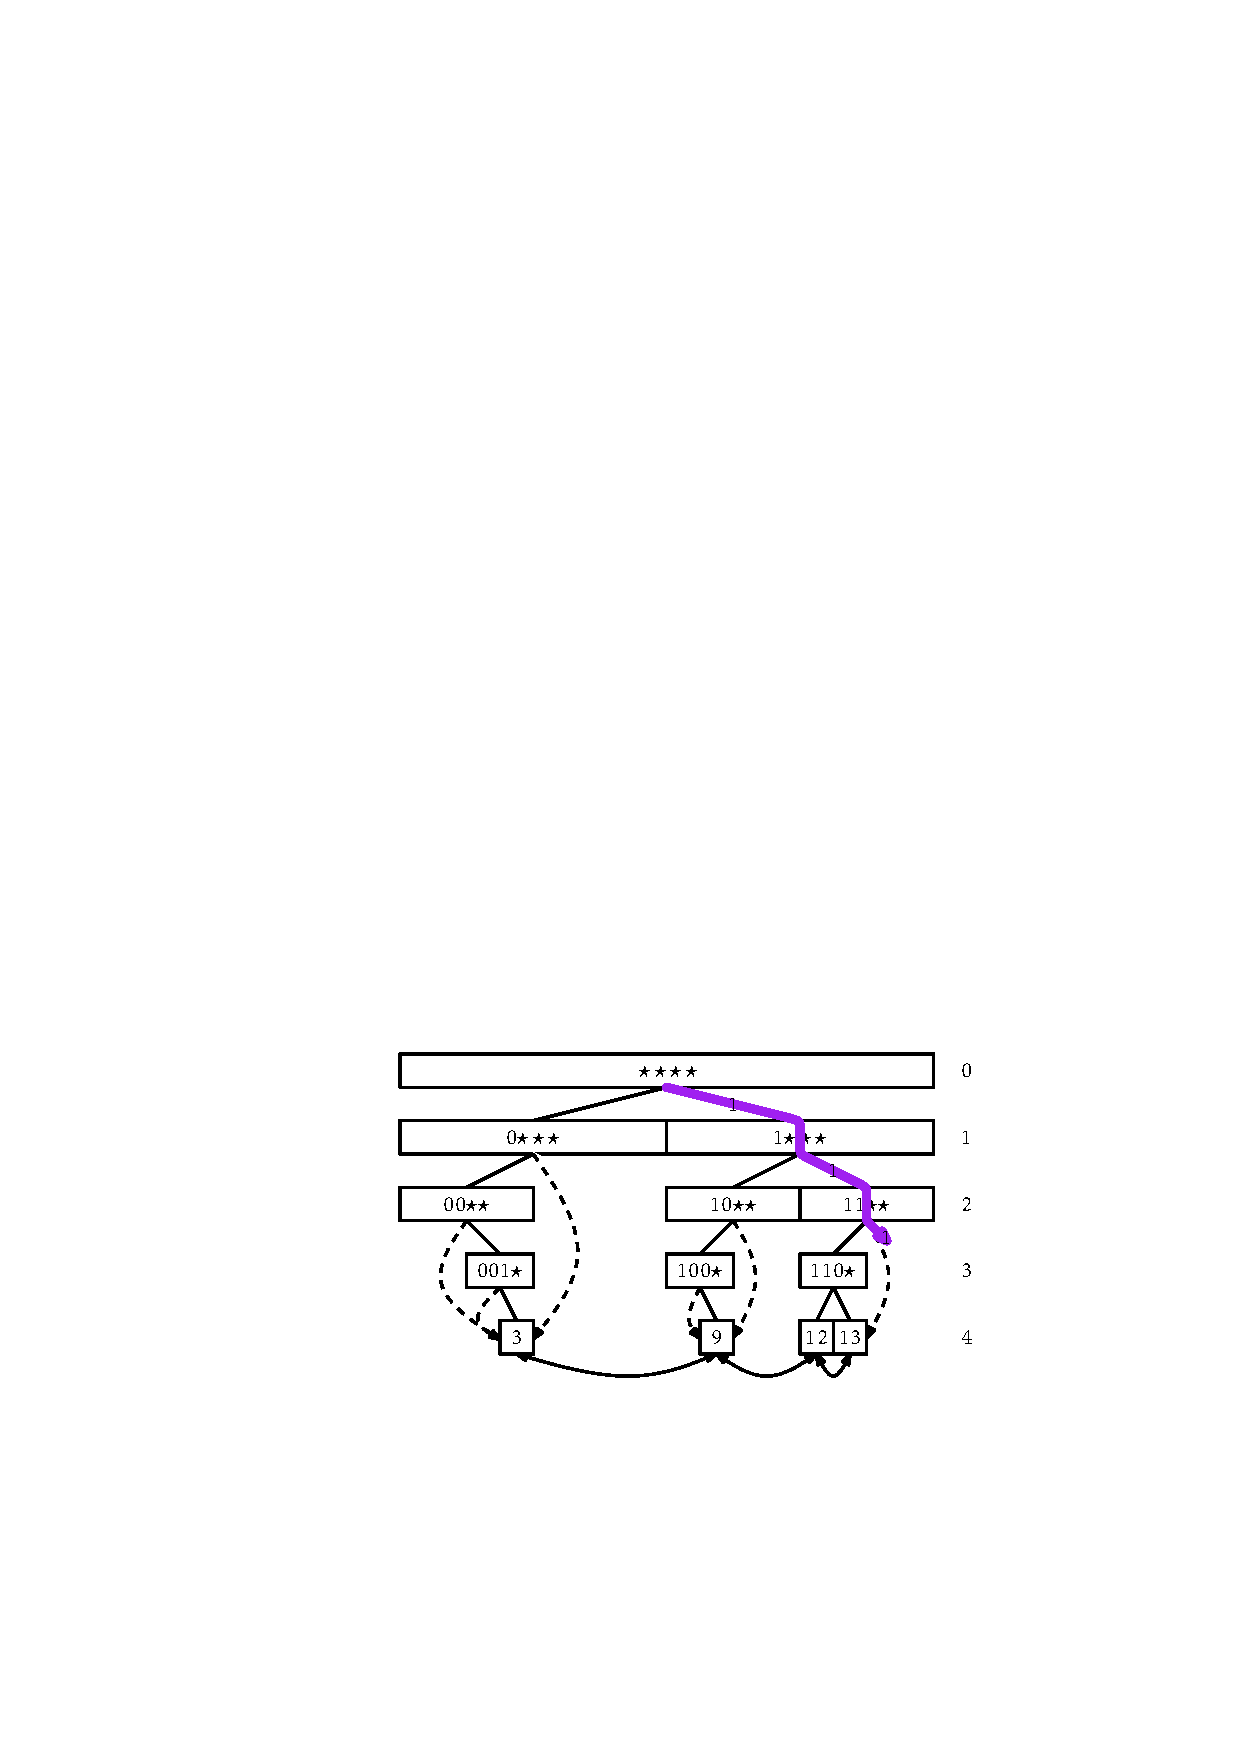
\includegraphics[scale=0.90909]{figs/xfast-path}
  \end{center}
  \caption{Since there is no node labelled $111\star$, the search path
    for 14 (1110) ends at the node labelled $11{\star\star}$ .}
  \figlabel{xfast-path}
\end{figure}

In an #XFastTrie#, we store, for each $#i#\in\{0,\ldots,#w#\}$, all
the nodes at level #i# in a #USet#, #t[i]#, that is implemented as a
hash table (\chapref{hashing}).  Using this #USet# allows us to check
in constant expected time if there is a node at level #i# whose label
matches the highest-order #i# bits of #x#.  In fact, we can even find
this node using
\javaonly{#t[i].find(x>>>(w-i))#}%
\cpponly{#t[i].find(x>>(w-i))#}%
\pcodeonly{#t[i].find(x>>(w-i))#}%

The hash tables $#t[0]#,\ldots,#t[w]#$ allow us to use binary search
to find #u#.  Initially, we know that #u# is at some level #i# with
$0\le #i#< #w#+1$. We therefore initialize $#l#=0$ and $#h#=#w#+1$
and repeatedly look at the hash table #t[i]#, where $#i#=\lfloor
(#l+h#)/2\rfloor$.  If $#t[i]#$ contains a node whose label matches
#x#'s highest-order #i# bits then we set #l=i# (#u# is at or below level
#i#); otherwise we set #h=i# (#u# is above level #i#).  This process
terminates when $#h-l#\le 1$, in which case we determine that #u# is
at level #l#.  We then complete the #find(x)# operation using #u.jump#
and the doubly-linked list of leaves.
\codeimport{ods/XFastTrie.find(x)}
Each iteration of the #while# loop in the above method decreases #h-l#
by roughly a factor of two, so this loop finds #u# after $O(\log #w#)$
iterations.  Each iteration performs a constant amount of work and one
#find(x)# operation in a #USet#, which takes a constant expected amount
of time.  The remaining work takes only constant time, so the #find(x)#
method in an #XFastTrie# takes only $O(\log#w#)$ expected time.

The #add(x)# and #remove(x)# methods for an #XFastTrie# are almost
identical to the same methods in a #BinaryTrie#.  The only modifications
are for managing the hash tables #t[0]#,\ldots,#t[w]#.  During the
#add(x)# operation, when a new node is created at level #i#, this node
is added to #t[i]#.  During a #remove(x)# operation, when a node is
removed form level #i#, this node is removed from #t[i]#.  Since adding
and removing from a hash table take constant expected time, this does
not increase the running times of #add(x)# and #remove(x)# by more than
a constant factor. We omit a code listing for #add(x)# and #remove(x)#
since the code is almost identical to the (long) code listing already
provided for the same methods in a #BinaryTrie#.

The following theorem summarizes the performance of an #XFastTrie#:

\begin{thm}
An #XFastTrie# implements the #SSet# interface for #w#-bit integers. An
#XFastTrie# supports the operations
\begin{itemize}
\item #add(x)# and #remove(x)# in $O(#w#)$ expected time per operation and 
\item #find(x)# in $O(\log #w#)$ expected time per operation.
\end{itemize}
The space used by an #XFastTrie# that
stores #n# values is $O(#n#\cdot#w#)$.
\end{thm}

\section{#YFastTrie#: A Doubly-Logarithmic Time #SSet#}
\seclabel{yfast}

The #XFastTrie# is a vast---even exponential---improvement over the
#BinaryTrie# in terms of query time, but the #add(x)# and #remove(x)#
operations are still not terribly fast.  Furthermore, the space usage,
$O(#n#\cdot#w#)$, is higher than the other #SSet# implementations
described in this book, which all use $O(#n#)$ space.  These two
problems are related; if #n# #add(x)# operations build a structure of
size $#n#\cdot#w#$, then the #add(x)# operation requires at least on the
order of #w# time (and space) per operation.

\index{YFastTrie@#YFastTrie#}%
The #YFastTrie#, discussed next, simultaneously improves the space and
speed of #XFastTrie#s.  A #YFastTrie# uses an #XFastTrie#, #xft#, but only
stores $O(#n#/#w#)$ values in #xft#.  In this way, the total space used by
#xft# is only $O(#n#)$.  Furthermore, only one out of every #w# #add(x)#
or #remove(x)# operations in the #YFastTrie# results in an #add(x)# or
#remove(x)# operation in #xft#.  By doing this, the average cost incurred
by calls to #xft#'s #add(x)# and #remove(x)# operations is only constant.

The obvious question becomes:  If #xft# only stores #n#/#w# elements,
where do the remaining $#n#(1-1/#w#)$ elements go?  These elements move 
into \emph{secondary structures},
\index{secondary structure}%
in this case an extended version of
treaps (\secref{treap}).  There are roughly #n#/#w# of these secondary
structures so, on average, each of them stores $O(#w#)$ items.  Treaps
support logarithmic time #SSet# operations, so the operations on these
treaps will run in $O(\log #w#)$ time, as required.

More concretely, a #YFastTrie# contains an #XFastTrie#, #xft#,
that contains a random sample of the data, where each element
appears in the sample independently with probability $1/#w#$.
For convenience, the value $2^{#w#}-1$, is always contained in #xft#.
Let $#x#_0<#x#_1<\cdots<#x#_{k-1}$ denote the elements stored in #xft#.
Associated with each element, $#x#_i$, is a treap, $#t#_i$, that stores
all values in the range $#x#_{i-1}+1,\ldots,#x#_i$.  This is illustrated
in \figref{yfast}.

\begin{figure}
  \begin{center}
    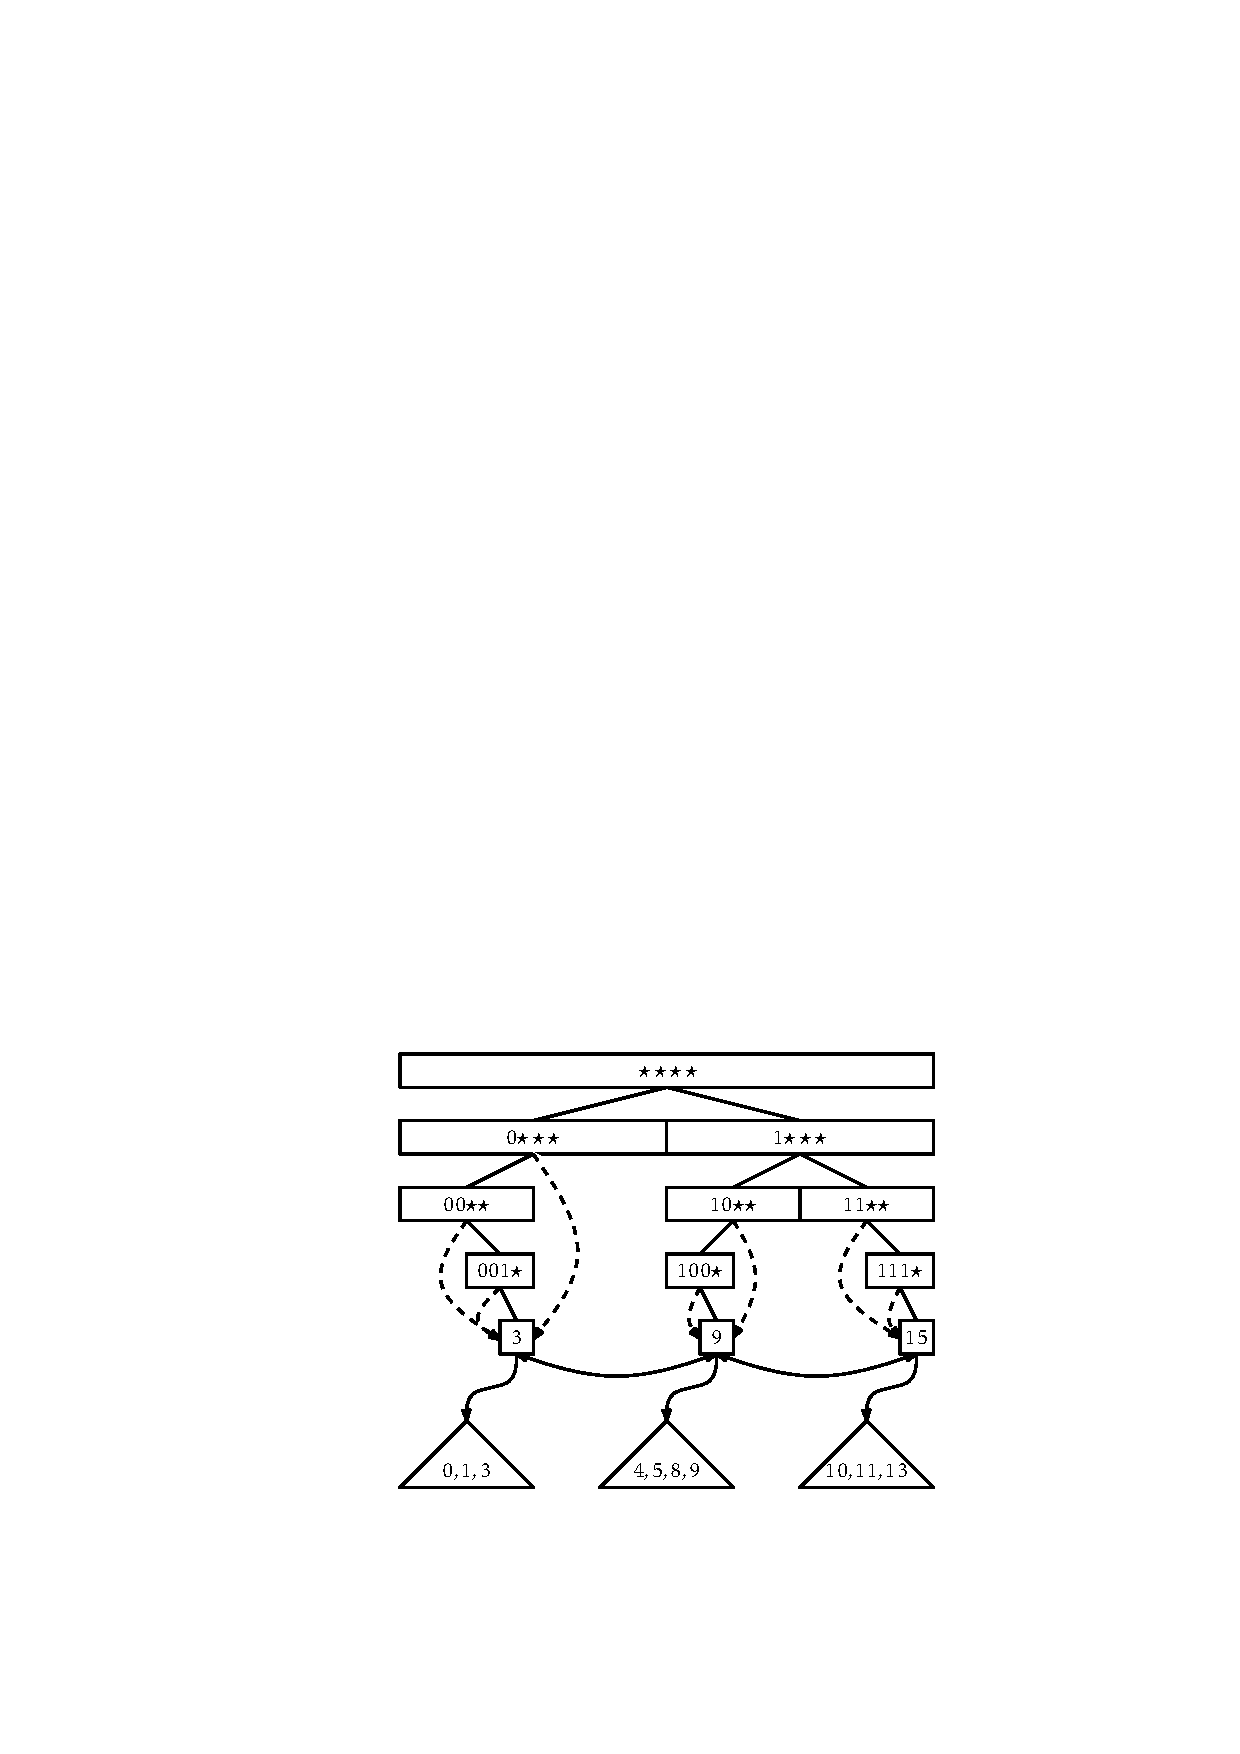
\includegraphics[scale=0.90909]{figs/yfast}
  \end{center}
  \caption[A YFastTrie]{A #YFastTrie# containing the values 0, 1, 3, 4,
  6, 8, 9, 10, 11, and 13.}
  \figlabel{yfast}
\end{figure}

The #find(x)# operation in a #YFastTrie# is fairly easy.  We search
for #x# in #xft# and find some value $#x#_i$ associated with the treap
$#t#_i$.  We then use the treap #find(x)# method on $#t#_i$ to answer
the query.  The entire method is a one-liner:
\codeimport{ods/YFastTrie.find(x)} 
The first #find(x)# operation (on #xft#) takes $O(\log#w#)$ time.
The second #find(x)# operation (on a treap) takes $O(\log r)$ time, where
$r$ is the size of the treap.  Later in this section, we will show that
the expected size of the treap is $O(#w#)$ so that this operation takes
$O(\log #w#)$ time.\footnote{This is an application of \emph{Jensen's Inequality}: If $\E[r]=#w#$, then $\E[\log r]
\le \log w$.}

Adding an element to a #YFastTrie# is also fairly simple---most of
the time.  The #add(x)# method calls #xft.find(x)# to locate the treap,
#t#, into which #x# should be inserted.  It then calls #t.add(x)# to
add #x# to #t#.  At this point, it tosses a biased coin that comes up as
heads with probability $1/#w#$ and as tails with probability $1-1/#w#$.
If this coin comes up heads, then #x# will be added to #xft#.

This is where things get a little more complicated.  When #x# is added to
#xft#, the treap #t# needs to be split into two treaps, #t1# and #t'#.
The treap #t1# contains all the values less than or equal to #x#;
#t'# is the original treap, #t#, with the elements of #t1# removed.
Once this is done, we add the pair #(x,t1)# to #xft#.  \figref{yfast-add}
shows an example.
\codeimport{ods/YFastTrie.add(x)}
\begin{figure}
  \begin{center}
    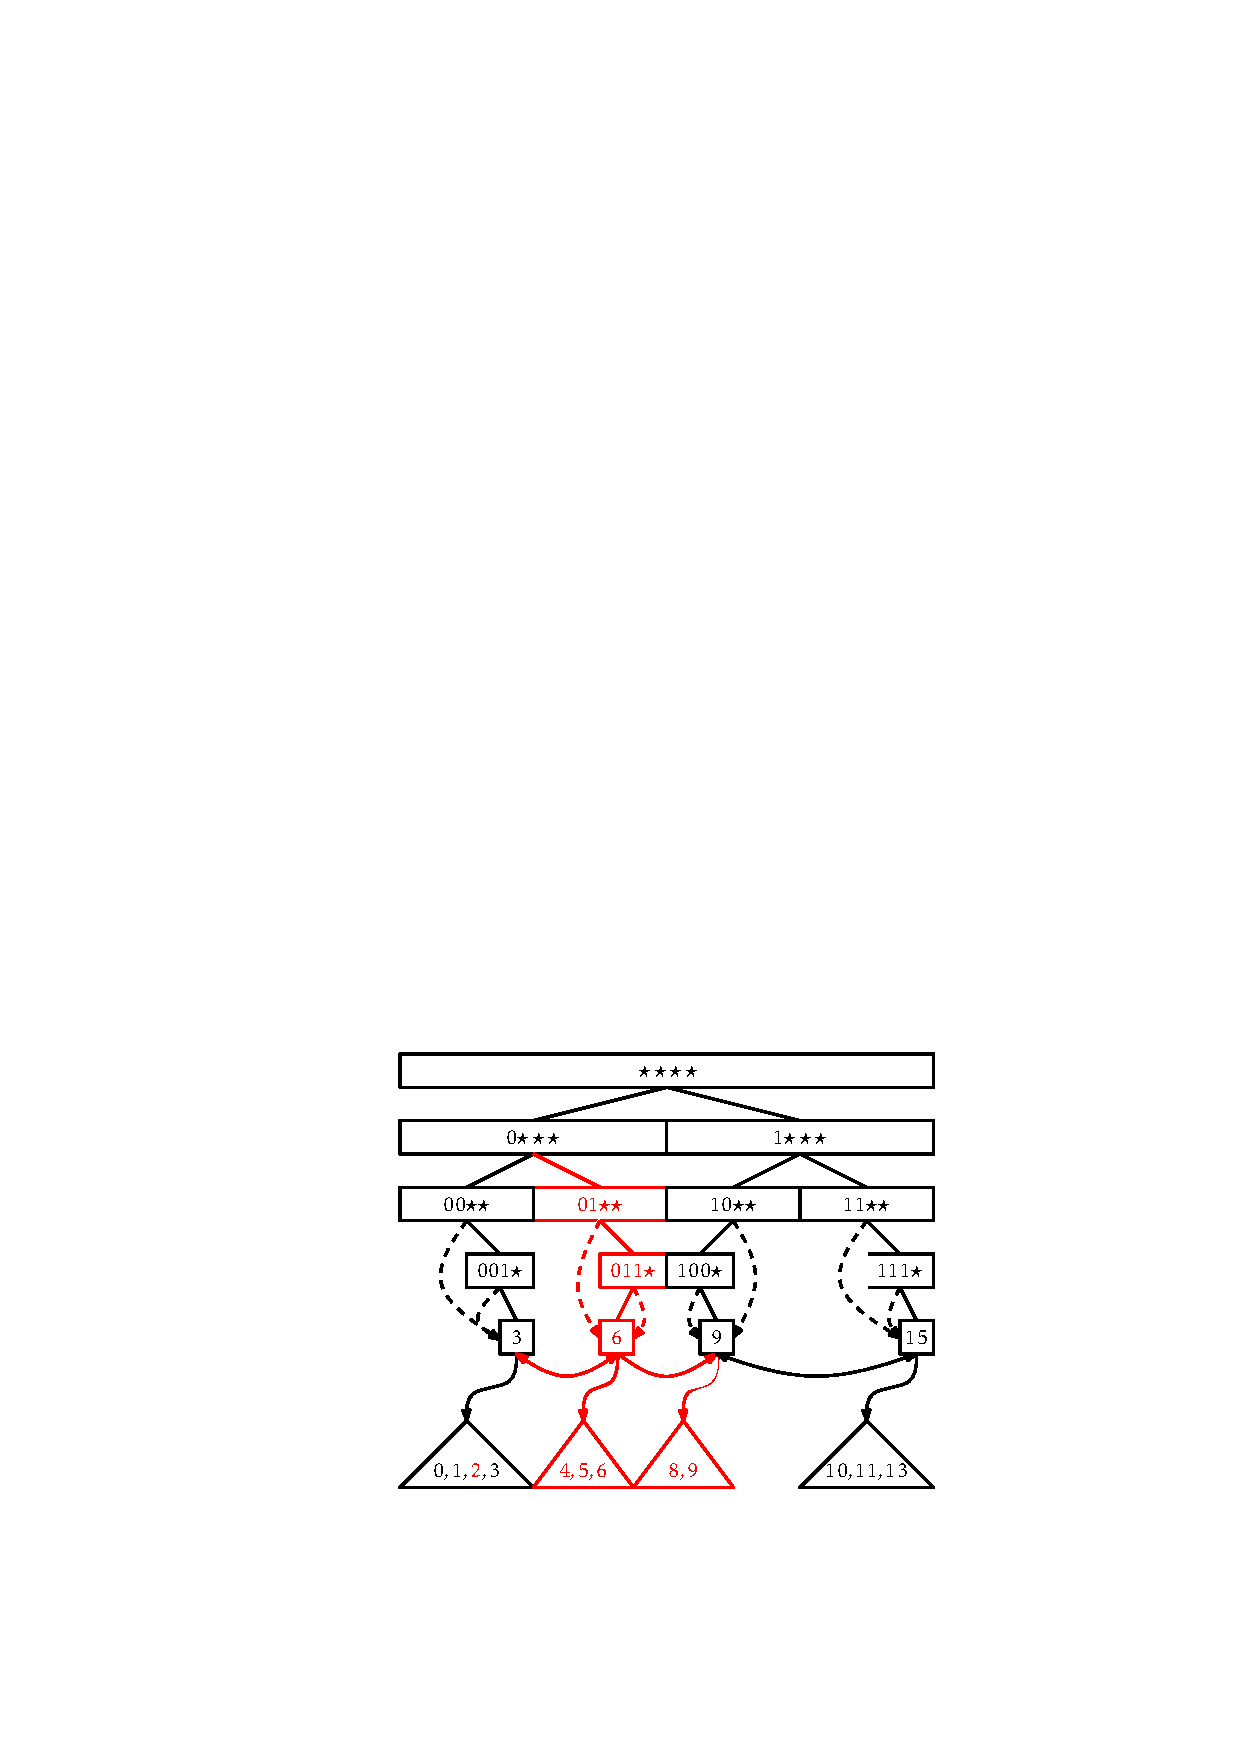
\includegraphics[scale=0.90909]{figs/yfast-add}
  \end{center}
  \caption[Adding to a YFastTrie]{Adding the values 2 and 6 to a #YFastTrie#. The coin toss
    for 6 came up heads, so 6 was added to #xft# and the treap containing
    $4,5,6,8,9$ was split.}
  \figlabel{yfast-add}
\end{figure}
Adding #x# to #t# takes $O(\log #w#)$ time.  \excref{treap-split} shows
that splitting #t# into #t1# and #t'# can also be done in $O(\log #w#)$
expected time.  Adding the pair (#x#,#t1#) to #xft# takes $O(#w#)$ time,
but only happens with probability $1/#w#$.  Therefore, the expected
running time of the #add(x)# operation is
\[
    O(\log#w#) + \frac{1}{#w#}O(#w#) = O(\log #w#) \enspace .
\]

The #remove(x)# method undoes the work performed by #add(x)#.
We use #xft# to find the leaf, #u#, in #xft# that contains the answer
to #xft.find(x)#.  From #u#, we get the treap, #t#, containing #x#
and remove #x# from #t#.  If #x# was also stored in #xft# (and #x#
is not equal to $2^{#w#}-1$) then we remove #x# from #xft# and add the
elements from #x#'s treap to the treap, #t2#, that is stored by #u#'s
successor in the linked list.   This is illustrated in
\figref{yfast-remove}.
\codeimport{ods/YFastTrie.remove(x)}
\begin{figure}
  \begin{center}
    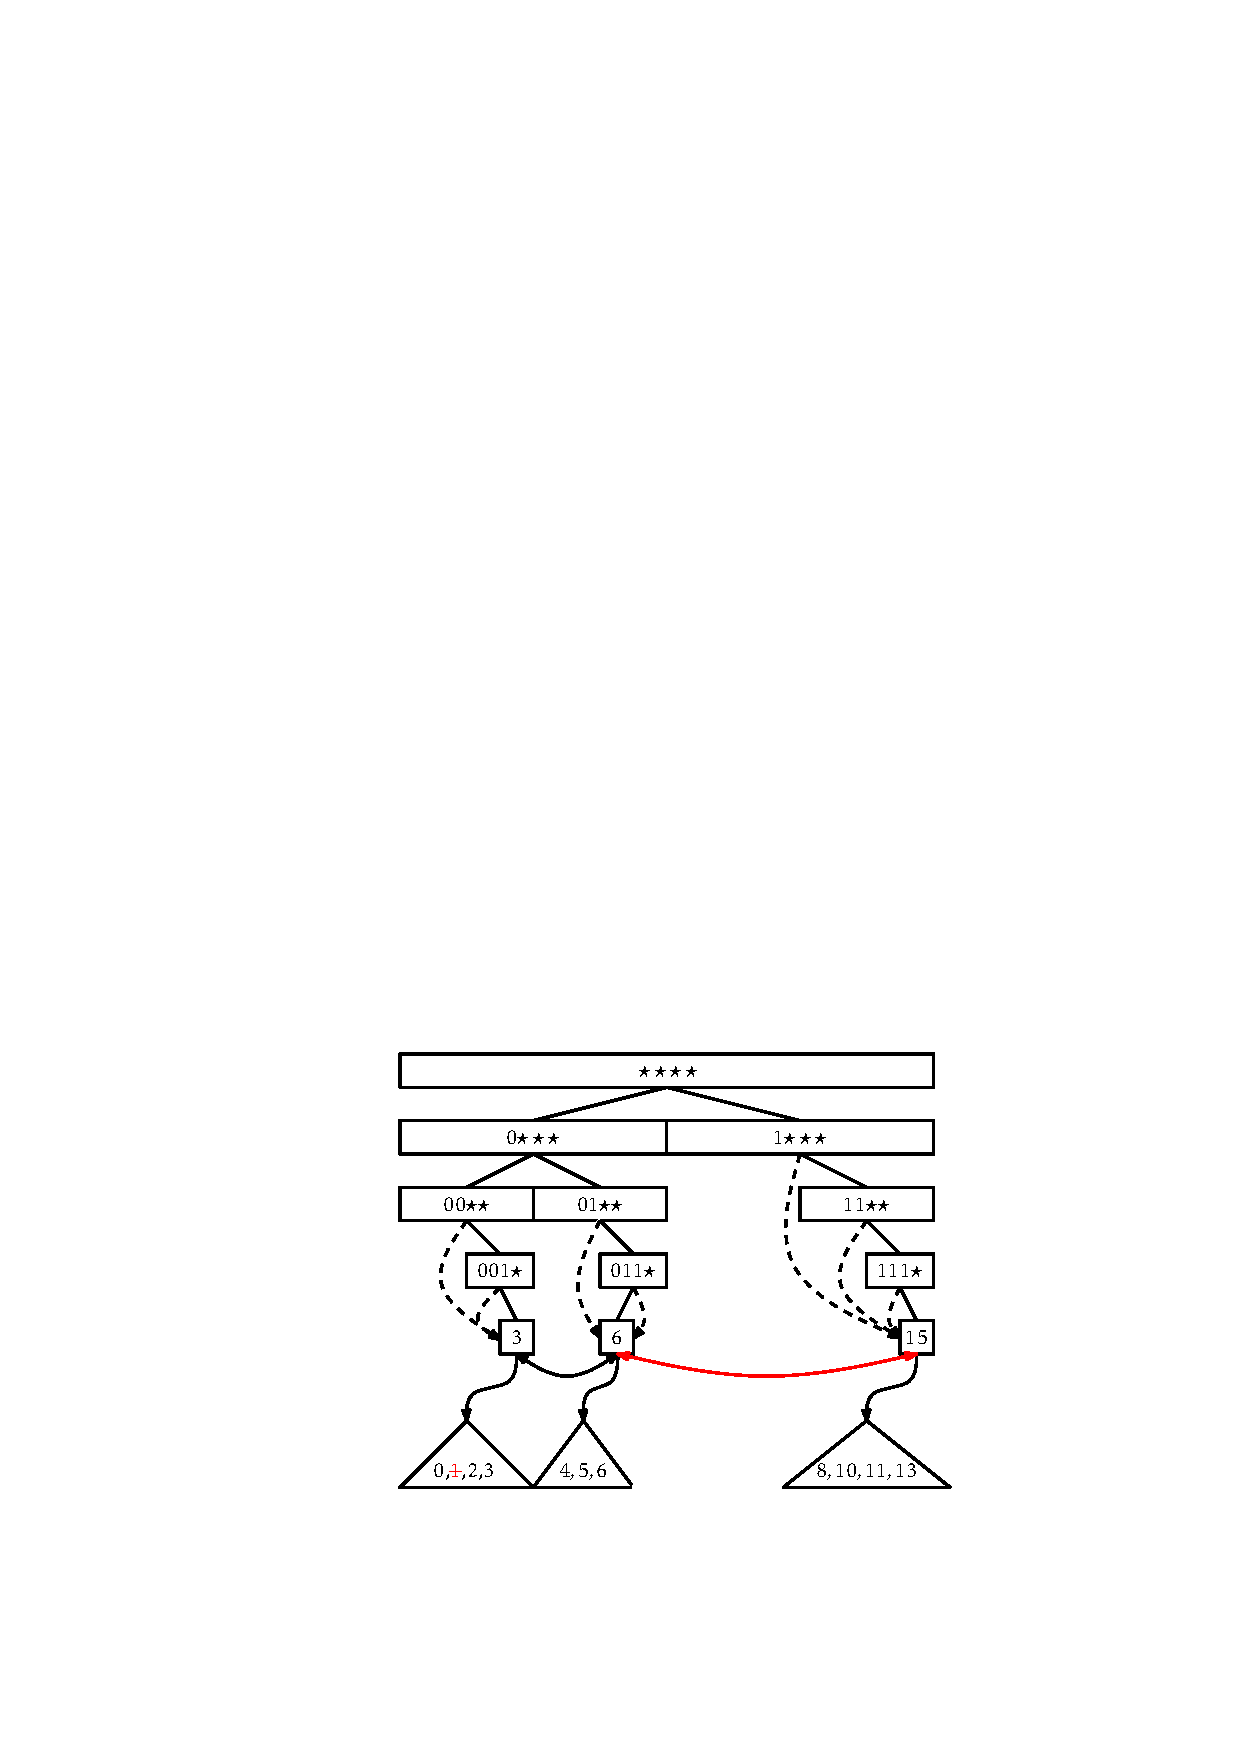
\includegraphics[scale=0.90909]{figs/yfast-remove}
  \end{center}
  \caption[Removing from a YFastTrie]{Removing the values 1 and 9 from a #YFastTrie# in \figref{yfast-add}.}
  \figlabel{yfast-remove}
\end{figure}
Finding the node #u# in #xft# takes $O(\log#w#)$ expected time.
Removing #x# from #t# takes $O(\log#w#)$ expected time.  Again,
\excref{treap-split} shows that merging all the elements of #t# into
#t2# can be done in $O(\log#w#)$ time.  If necessary, removing #x#
from #xft# takes $O(#w#)$ time, but #x# is only contained in #xft# with
probability $1/#w#$.  Therefore, the expected time to remove an element
from a #YFastTrie# is $O(\log #w#)$.

Earlier in the discussion, we delayed arguing about the sizes of treaps
in this structure until later.  Before finishing this chapter, we prove
the result we need.

\begin{lem}\lemlabel{yfast-subtreesize}
Let #x# be an integer stored in a #YFastTrie# and let $#n#_#x#$
denote the number of elements in the treap, #t#, that contains #x#.
Then $\E[#n#_#x#] \le 2#w#-1$.
\end{lem}

\begin{proof}
Refer to \figref{yfast-sample}. Let
$#x#_1<#x#_2<\cdots<#x#_i=#x#<#x#_{i+1}<\cdots<#x#_#n#$ denote
the elements stored
in the #YFastTrie#.  The treap #t# contains some elements greater than
or equal to #x#.  These are $#x#_i,#x#_{i+1},\ldots,#x#_{i+j-1}$,
where $#x#_{i+j-1}$ is the only one of these elements in which the
biased coin toss performed in the #add(x)# method turned up as heads.
In other words, $\E[j]$ is equal to the expected number of biased coin
tosses required to obtain the first heads.\footnote{This analysis ignores
the fact that $j$ never exceeds $#n#-i+1$.  However, this only decreases
$\E[j]$, so the upper bound still holds.}  Each coin toss is independent
and turns up as heads with probability $1/#w#$, so $\E[j]\le#w#$.
(See \lemref{coin-tosses} for an analysis of this for the case $#w#=2$.)

Similarly, the elements of #t# smaller than #x# are
$#x#_{i-1},\ldots,#x#_{i-k}$ where all these $k$ coin tosses turn up as
tails and the coin toss for $#x#_{i-k-1}$ turns up as heads.  Therefore,
$\E[k]\le#w#-1$, since this is the same coin tossing experiment considered
in the preceding paragraph, but one in which the last toss is not counted.
In summary, $#n#_#x#=j+k$, so
\[  \E[#n#_#x#] = \E[j+k] = \E[j] + \E[k] \le 2#w#-1 \enspace .  \qedhere \]
\end{proof}
\begin{figure}
  \begin{center}
    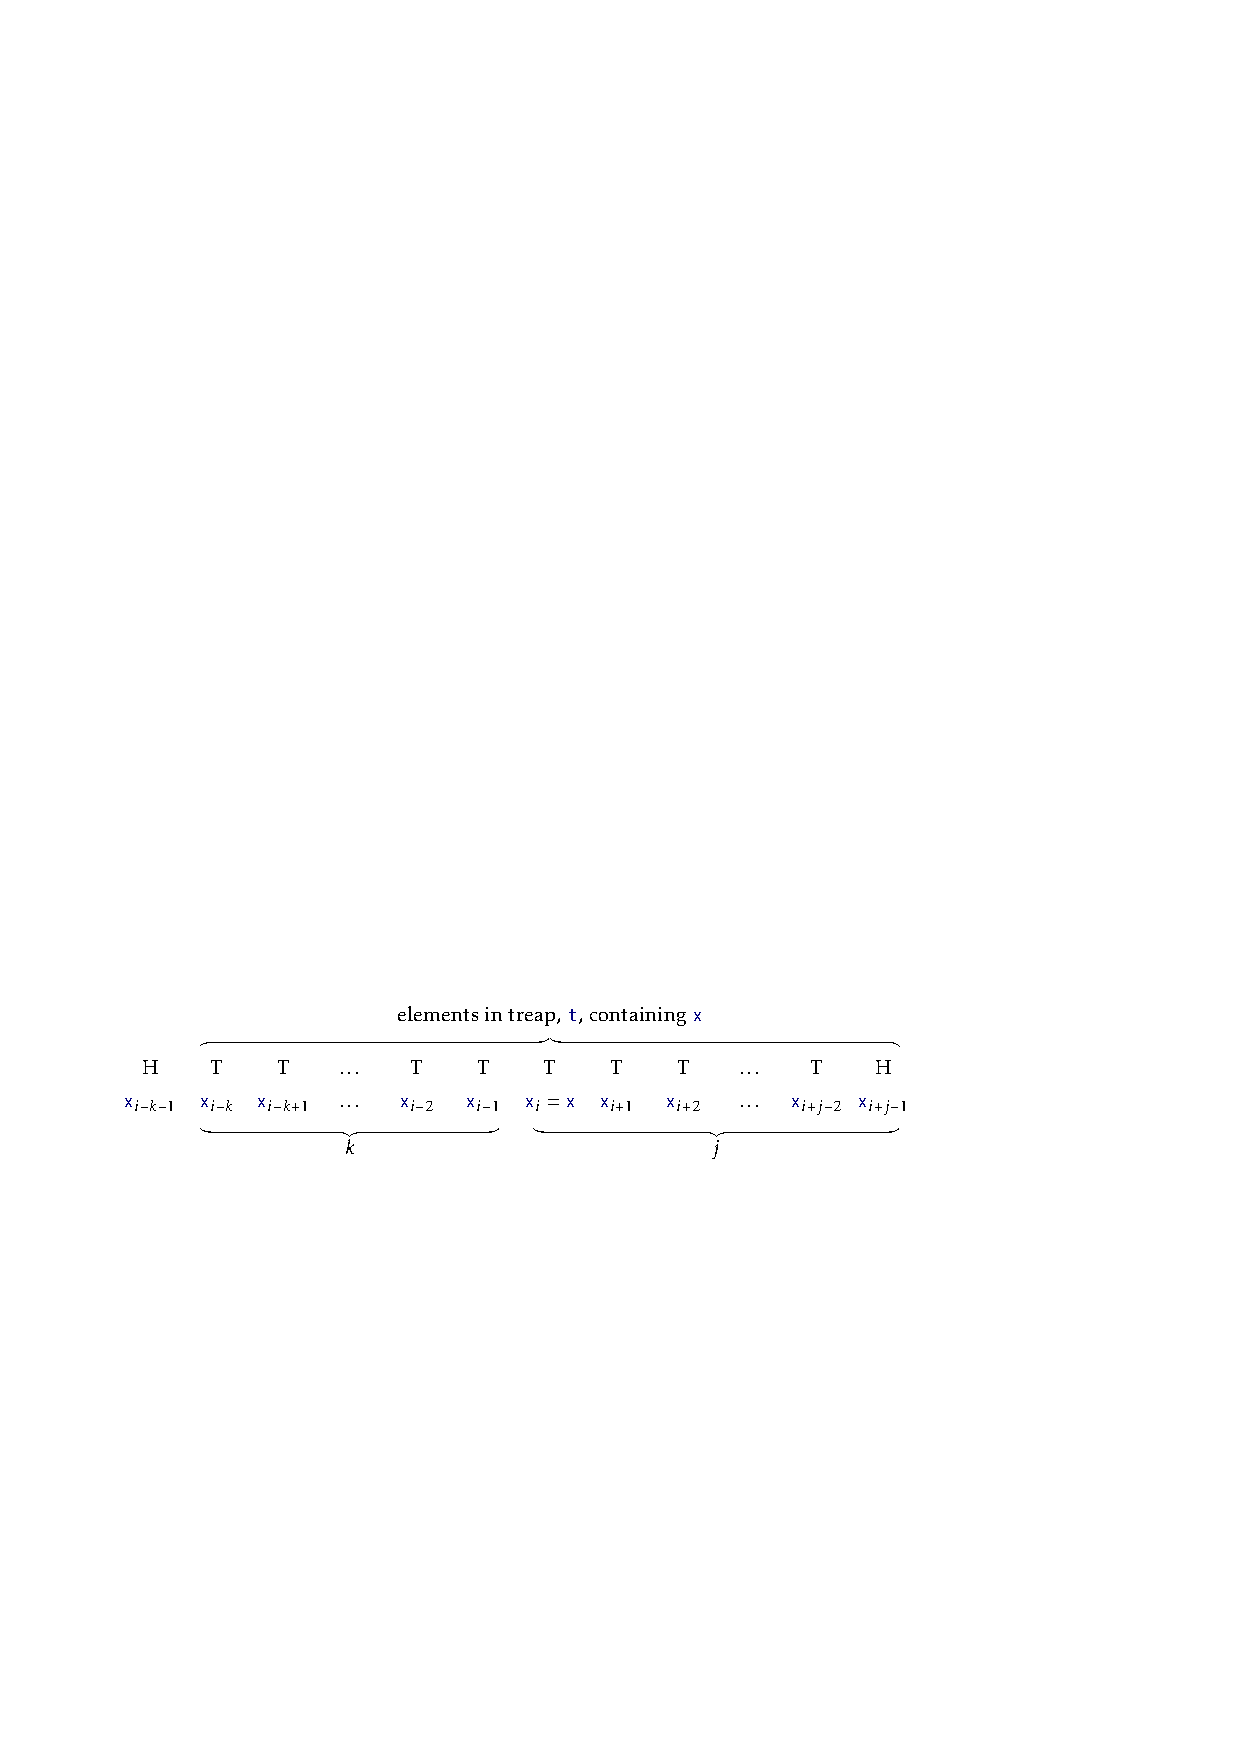
\includegraphics[width=\ScaleIfNeeded]{figs/yfast-sample}
  \end{center}
  \caption[The query time in a YFastTrie]{The number of elements in
  the treap #t# containing #x# is determined by two coin tossing
  experiments.}
  \figlabel{yfast-sample}
\end{figure}
%Surprisingly, the bound in \lemref{yfast-subtreesize} is tight.  (If this
%isn't surprising to the reader, they can stop reading this paragraph now.)
%This is counterintuitive because #xft# contains any particular element
%with probability $1/#w#$ so it contains about $n/#w#$ elements.  In other
%words, the average number of elements assigned to one treap is #w#.
%\lemref{yfast-subtreesize} says that the expected size of the treap that
%contains #x# is about twice as large as the average.  This seeming
%discrepancy comes from the fact that larger subtrees contain more elements
%and therefore #x# is more likely to be in a larger subtree than a smaller
%one.

\lemref{yfast-subtreesize} was the last piece in the proof of the
following theorem, which summarizes the performance of the #YFastTrie#:

\begin{thm}
A #YFastTrie# implements the #SSet# interface for #w#-bit integers. A
#YFastTrie# supports the operations #add(x)#, #remove(x)#, and #find(x)#
in $O(\log #w#)$ expected time per operation.  The space used by a
#YFastTrie# that stores #n# values is $O(#n#+#w#)$.
\end{thm}

The #w# term in the space requirement comes from the fact that #xft# always
stores the value $2^#w#-1$.  The implementation could be modified (at the
expense of adding some extra cases to the code) so that it is unnecessary
to store this value.  In this case, the space requirement in the theorem
becomes $O(#n#)$.

\section{Discussion and Exercises}

The first data structure to provide $O(\log#w#)$ time #add(x)#,
#remove(x)#, and #find(x)# operations was proposed by van~Emde~Boas and
has since become known as the \emph{van~Emde~Boas}
\index{van Emde Boas tree}%
(or \emph{stratified})
\index{stratified tree}%
\emph{tree} \cite{e77}.  The original van~Emde~Boas structure had size
$2^{#w#}$, making it impractical for large integers.

The #XFastTrie# and #YFastTrie# data structures were discovered by
Willard \cite{w83}.  The #XFastTrie# structure is closely related
to van~Emde~Boas trees;  for instance, the hash tables in an #XFastTrie#
replace arrays in a van~Emde~Boas tree.  That is, instead of storing
the hash table #t[i]#, a van~Emde~Boas tree stores an array of length
$2^{#i#}$.

Another structure for storing integers is Fredman and Willard's fusion
trees \cite{fw93}.
\index{fusion tree}%
This structure can store #n# #w#-bit integers in
$O(#n#)$ space so that the #find(x)# operation runs in $O((\log #n#)/(\log
#w#))$ time.  By using a fusion tree when $\log #w# > \sqrt{\log #n#}$ and
a #YFastTrie# when $\log #w# \le \sqrt{\log #n#}$, one obtains an $O(#n#)$
space data structure that can implement the #find(x)# operation in
$O(\sqrt{\log #n#})$ time.  Recent lower-bound results of P\v{a}tra\c{s}cu
and Thorup \cite{pt07} show that these results are more or less optimal,
at least for structures that use only $O(#n#)$ space.

\begin{exc}
  Design and implement a simplified version of a #BinaryTrie# that
  does not have a linked list or jump pointers, but for which #find(x)#

  still runs in $O(#w#)$ time.
\end{exc}

\begin{exc}
  Design and implement a simplified implementation of an #XFastTrie#
  that doesn't use a binary trie at all. Instead, your implementation
  should store everything in a doubly-linked list and $#w#+1$
  hash tables.
\end{exc}

\begin{exc}
  We can think of a #BinaryTrie# as a structure that stores bit strings
  of length #w# in such a way that each bitstring is represented as a
  root to leaf path.  Extend this idea into an #SSet# implementation that
  stores variable-length strings and implements #add(s)#, #remove(s)#,
  and #find(s)# in time proporitional to the length of #s#.

  \noindent Hint: Each node in your data structure should store a hash
  table that is indexed by character values.
\end{exc}

\begin{exc}
  For an integer $#x#\in\{0,\ldots2^{#w#}-1\}$, let $d(#x#)$ denote
  the difference between #x# and the value returned by #find(x)#
  [if #find(x)# returns #null#, then define $d(#x#)$ as $2^#w#$].
  For example, if #find(23)# returns 43, then $d(23)=20$.
  \begin{enumerate}
    \item Design and implement a modified version of the #find(x)#
      operation in an #XFastTrie# that runs in $O(1+\log d(#x#))$
      expected time. Hint: The hash table $t[#w#]$ contains all the
      values, #x#, such that $d(#x#)=0$, so that would be a good place
      to start.
    \item Design and implement a modified version of the #find(x)#
      operation in an  #XFastTrie# that runs in $O(1+\log\log d(#x#))$
      expected time.
  \end{enumerate}
\end{exc}


